\documentclass[10pt,twocolumn,letterpaper]{article}

\usepackage{cvpr}
\usepackage{times}
\usepackage{epsfig}
\usepackage{graphicx}
\usepackage{amsmath}
\usepackage{amssymb}
\usepackage{tikz}
\usepackage{pgfplots}
\usetikzlibrary{shadows,trees}

\usepackage{verbatim}
\usepackage{bm}
\usepackage{microtype}
\usepackage{url}
\usepackage{multirow}
\usepackage{caption}
\usepackage{subcaption}
\usepackage{booktabs} % for better tables
\usepackage{microtype}

\newlength{\eqs}
\setlength{\eqs}{-0.04in}

\usepackage{enumitem}
\setitemize[0]{leftmargin=15pt}

\newenvironment{tight_itemize}{
\begin{itemize}[leftmargin=10pt]
  \setlength{\topsep}{0pt}
  \setlength{\itemsep}{0pt}
  \setlength{\parskip}{0pt}
  \setlength{\parsep}{0pt}
}{\end{itemize}}



% If you comment hyperref and then uncomment it, you should delete
% egpaper.aux before re-running latex.  (Or just hit 'q' on the first latex
% run, let it finish, and you should be clear).
\usepackage[pagebackref=true,breaklinks=true,letterpaper=true,colorlinks,bookmarks=false]{hyperref}


% New math commands/abreviations

\newcommand{\bA}{\mathbf{A}}
\newcommand{\bB}{\mathbf{B}}
\newcommand{\bC}{\mathbf{C}}
\newcommand{\bD}{\mathbf{D}}
\newcommand{\bE}{\mathbf{E}}
\newcommand{\bF}{\mathbf{F}}
\newcommand{\bG}{\mathbf{G}}
\newcommand{\bH}{\mathbf{H}}
\newcommand{\bI}{\mathbf{I}}
\newcommand{\bJ}{\mathbf{J}}
\newcommand{\bK}{\mathbf{K}}
\newcommand{\bL}{\mathbf{L}}
\newcommand{\bM}{\mathbf{M}}
\newcommand{\bN}{\mathbf{N}}
\newcommand{\bO}{\mathbf{O}}
\newcommand{\bP}{\mathbf{P}}
\newcommand{\bQ}{\mathbf{Q}}
\newcommand{\bR}{\mathbf{R}}
\newcommand{\bS}{\mathbf{S}}
\newcommand{\bT}{\mathbf{T}}
\newcommand{\bU}{\mathbf{U}}
\newcommand{\bV}{\mathbf{V}}
\newcommand{\bW}{\mathbf{W}}
\newcommand{\bX}{\mathbf{X}}
\newcommand{\bY}{\mathbf{Y}}
\newcommand{\bZ}{\mathbf{Z}}

\newcommand{\ba}{\mathbf{a}}
%\newcommand{\bb}{\mathbf{b}}
\newcommand{\bc}{\mathbf{c}}
\newcommand{\bd}{\mathbf{d}}
\newcommand{\be}{\mathbf{e}}
%\newcommand{\bf}{\mathbf{f}}
\newcommand{\bg}{\mathbf{g}}
\newcommand{\bh}{\mathbf{h}}
\newcommand{\bi}{\mathbf{i}}
\newcommand{\bj}{\mathbf{j}}
\newcommand{\bk}{\mathbf{k}}
\newcommand{\bl}{\mathbf{l}}
%\newcommand{\bm}{\mathbf{m}}
\newcommand{\bn}{\mathbf{n}}
%\newcommand{\bo}{\mathbf{o}}
\newcommand{\bp}{\mathbf{p}}
\newcommand{\bq}{\mathbf{q}}
\newcommand{\br}{\mathbf{r}}
\newcommand{\bs}{\mathbf{s}}
\newcommand{\bt}{\mathbf{t}}
\newcommand{\bu}{\mathbf{u}}
\newcommand{\bv}{\mathbf{v}}
\newcommand{\bw}{\mathbf{w}}
\newcommand{\bx}{\mathbf{x}}
\newcommand{\by}{\mathbf{y}}
\newcommand{\bz}{\mathbf{z}}

\newcommand{\bff}{\mathbf{f}}

\newcommand{\bo}{\mathbf{0}}
\newcommand{\tx}{\tilde{\mathbf{x}}}


\newcommand{\hbn}{{\widehat{\mathbf{n}}}}
\newcommand{\hbs}{{\widehat{\mathbf{s}}}}
\newcommand{\hbh}{{\widehat{\mathbf{h}}}}
\newcommand{\hbv}{{\widehat{\mathbf{v}}}}
\newcommand{\hbw}{{\widehat{\mathbf{w}}}}
\newcommand{\hbc}{{\widehat{\mathbf{c}}}}

\newcommand{\hh}{{\widehat{h}}}
\newcommand{\hn}{{\widehat{n}}}
\newcommand{\hx}{{\widehat{x}}}
\newcommand{\hy}{{\widehat{y}}}
\newcommand{\hz}{{\widehat{z}}}


% Mathcal definitions
\newcommand{\cS}{\mathcal{S}}
\newcommand{\cD}{\mathcal{D}}
\newcommand{\cP}{{\mathcal{P}}}
\newcommand{\cU}{{\mathcal{U}}}
\newcommand{\cV}{{\mathcal{V}}}
\newcommand{\cE}{{\mathcal{E}}}
\newcommand{\cQ}{{\mathcal{Q}}}
\newcommand{\cG}{{\mathcal{G}}}
\newcommand{\cB}{{\mathcal{B}}}
\newcommand{\cI}{\mathcal{I}}
\newcommand{\cL}{\mathcal{L}}
\newcommand{\cR}{{\mathcal{R}}}
\newcommand{\cC}{{\mathcal{C}}}
\newcommand{\cO}{{\mathcal{O}}}
\newcommand{\cX}{{\mathcal{X}}}



% Mathbb definitions
\newcommand{\bbp}{\mathbb{P}}
\newcommand{\bbP}{\mathbb{P}}
\newcommand{\bbQ}{\mathbb{Q}}
\newcommand{\bbr}{\mathbb{R}}
\newcommand{\bbR}{\mathbb{R}}
\newcommand{\bbS}{\mathbb{S}}
\newcommand{\bbN}{\mathbb{N}}



% Mathbm definitions
\newcommand{\balpha}{{\bm{\alpha}}}
\newcommand{\bbeta}{{\bm{\beta}}}
\newcommand{\bgamma}{{\bm{\gamma}}}
\newcommand{\bepsilon}{{\bm{\epsilon}}}
\newcommand{\bmu}{{\bm{\mu}}}
\newcommand{\bpi}{\bm{\pi}}
\newcommand{\brho}{\bm{\rho}}
\newcommand{\bomega}{\bm{\omega}}
\newcommand{\bOmega}{\bm{\Omega}}
\newcommand{\bSigma}{\bm{\Sigma}}
\newcommand{\bGamma}{\bm{\Gamma}}



\newcommand{\id}{\mathbf{I}}
\newcommand{\tid}{\tilde{\id}}
\newcommand{\st}{{\textrm{subject to }}}


\newcommand{\bpm}{{\widehat{\bP}}}
\newcommand{\bxm}{{\widehat{\mathbf{X}}}}
\newcommand{\winf}{{{\bm{\Omega}}_\infty}}
%\newcommand{\bw}{{{\bm{\omega}}^*}}
\newcommand{\bwi}{{{\bm{\omega}}_i^*}}
\newcommand{\bwone}{{{\bm{\omega}}_1^*}}
\newcommand{\diac}{{{\bm{\omega}}^*}}
\newcommand{\iac}{{{\bm{\omega}}}}
\newcommand{\ac}{{{\bm{\Omega}}_\infty}}
\newcommand{\diaci}{{{\bm{\omega}}_i^*}}
\newcommand{\diacone}{{{\bm{\omega}}_1^*}}
\newcommand{\w}{{{\bm{\omega}}^*}}
\newcommand{\daq}{{\mathbf{Q}}_\infty^*}
\newcommand{\adq}{{\mathbf{Q}}_\infty^*}
\newcommand{\pinf}{{\bm{\pi}}_\infty}
\newcommand{\hinf}{{{\bH}_\infty}}
\newcommand{\hinft}{{{\bH}^\top_\infty}}
\newcommand{\hinfi}{{{\bH}^i_\infty}}
\newcommand{\hinfit}{{{\bH}^{i\top}_\infty}}
\newcommand{\hinfj}{{{\bH}^j_\infty}}
\newcommand{\hinfjt}{{{\bH}^{j\top}_\infty}}
\newcommand{\intval}[2]{[\, #1, #2 \, ]}
\newcommand{\camo}{\left[ \: \id \: \vert \: \bo \: \right]}
\newcommand{\cama}{\left[ \: \bA \: \vert \: \ba \: \right]}
\newcommand{\camr}{\left[ \: \bR \: \vert \: \bt \: \right]}
\newcommand{\camai}{\left[ \: \bA_i \: \vert \: \ba_i \: \right]}
\newcommand{\camri}{\left[ \: \bR_i \: \vert \: \bt_i \: \right]}

%\newcommand{\algorithmiccomment}[1]{//#1}
\newcommand{\lb}{\operatorname{\bf{Bound}}}
\newcommand{\branch}{\operatorname{\bf{Branch}}}
\newcommand{\feasible}{\operatorname{\bf{Feasible}}}
\newcommand{\trace}{\operatorname{Tr}}
\newcommand{\convenv}{\operatorname{\bf{convenv}}}
\newcommand{\rectangle}{Q}

\newcommand{\epi}{\operatorname{\bf{epi}}}
\newcommand{\dom}{\operatorname{\bf{dom}}}

\newcommand{\ophi}{f}
\newcommand{\phimin}{\ophi_{\text{min}}}
\newcommand{\philb}{\ophi_{\text{lb}}}
\newcommand{\phiub}{\ophi_{\text{ub}}}

\newcommand{\cvx}{{\mathrm{convex\_env}}}
\newcommand{\ccv}{{\mathrm{concave\_env}}}

\newcommand{\conc}[1]{\operatorname{conc}{#1}}
\newcommand{\conv}[1]{\operatorname{conv}{#1}}

%\newcommand{\deg}[1]{\operatorname{deg}{#1}}

\newcommand{\lmi}[1]{\operatorname{LMI}{#1}}

\newcommand{\fa}{\alpha}
\newcommand{\fb}{\beta}
\newcommand{\fc}{\gamma}


%\newcommand{\tr}{^\top}

\newcommand{\xlt}{x_l^{1/3}}
\newcommand{\xut}{x_u^{1/3}}
\newcommand{\tlt}{t_l^{1/3}}
\newcommand{\tut}{t_u^{1/3}}
\newcommand{\xl}{x_l}
\newcommand{\xu}{x_u}
\newcommand{\yl}{y_l}
\newcommand{\yu}{y_u}
\newcommand{\tl}{t_l}
\newcommand{\tu}{t_u}
\newcommand{\yp}{y_p}
\newcommand{\ypd}{y'_p}
\newcommand{\tp}{t_p}
\newcommand{\fl}{\frac{x - \xl}{\xu - \xl}}
\newcommand{\fu}{\frac{\xu - x}{\xu - \xl}}


% Bilinear definitions
\newcommand{\cl}{{\psi}^l}
\newcommand{\cu}{{\psi}^u}
\newcommand{\rect}{Q}
\newcommand{\cond}[1]{\operatorname{{\mathcal{C}}}{#1}}
\newcommand{\vol}[1]{\operatorname{vol}{#1}}

%\newcommand{\phimin}[1]{\operatorname{\Phi_{\textrm{min}}}{#1}}
%\newcommand{\philb}[1]{\operatorname{\Phi_{\textrm{lb}}}{#1}}
%\newcommand{\phiub}[1]{\operatorname{\Phi_{\textrm{ub}}}{#1}}


%\newcommand{\rank}{{\mathbf{rank}}}
%\newcommand{\diag}{{\mathrm{diag}}}

\newcommand{\rank}[1]{\operatorname{rank}{#1}}

%\newcommand{\bx}{x} %general unknown x
%\newcommand{\bX}{X} %scene point

\newcommand{\ix}{\bx} %image point
\newcommand{\ixa}{u} %1st coordinate of image point
\newcommand{\ixb}{v} %2nd coordinate of image point
\newcommand{\bXa}{U} %1st coordinate of scene point
\newcommand{\bXb}{V} %2nd coordinate of scene point
\newcommand{\bXc}{W} %3rd coordinate of scene point

\newcommand{\tr}{^\top}

\newcommand{\Linf}{L_{\infty}}
\newcommand{\Ltwo}{L_{2}}
\newcommand{\Lone}{L_{1}}
\newcommand{\Lp}{L_{p}}
\newcommand{\Lq}{L_{q}}

\def\smallmat#1{\left[\begin{smallmatrix}#1\end{smallmatrix}\right]}



\newcommand{\brs}{\bR_0}
\newcommand{\bts}{\bt_0}
\newcommand{\bzero}{\mathbf{0}}
\newcommand{\bdx}{\mathbf{dx}}

\newcommand{\p}{\partial}


\newcommand{\del}[1]{\nabla_{#1}}
\newcommand{\I}{\mathbf{I}}
\newcommand{\II}{\mathbf{II}}
\newcommand{\skewsymm}[1]{[{#1}]_\times}





% 3D pose of the cars and ego motion
\newcommand{\pos}[2]{\mathbf{p}^{#1}({#2})}
\newcommand{\ori}[2]{\mathbf{\omega}^{#1}(#2)}
\newcommand{\state}[2]{\mathbf{s}^{#1}(#2)}

% ego pose
\newcommand{\egop}[1][t]{\pos{c}{#1}}
\newcommand{\egoo}[1][t]{\ori{c}{#1}}
\newcommand{\egos}[1][t]{\state{c}{#1}}

% relative pose between camera and car $i$
\newcommand{\relp}[2]{\Omega^{#1}(#2)}
\newcommand{\relpz}[2]{\Omega_z^{#1}(#2)}

% 3D tracks on car $i$ in its own coordinate frame
\newcommand{\tracklets}{\mathbf{X}^{i}_o}
\newcommand{\tracklet}[1]{\mathbf{x}^{i}_{#1}}
% track projections on camera
\newcommand{\trackpit}[2]{\mathbf{u}_{#1}(#2)}
\newcommand{\trackp}[1]{\mathbf{u}_j(#1)}
\newcommand{\trackpj}[1]{\mathbf{u}_j(#1)}
% Unclassified track point projected on camera
\newcommand{\ucTrackp}{\mathbf{u}(t)}


% dimensions of car $i$
\newcommand{\dimsn}[1]{\mathbf{B}^{#1}}
\newcommand{\expDimsn}{\hat{\mathbf{B}}}

% projection function
\newcommand{\projectionOf}[1]{\pi_{\relp{i}{t}}\left(#1\right)}
\newcommand{\projectionOft}[1]{\pi_{\relp{i}{t+1}}\left(#1\right)}
\newcommand{\centerProj}{\bar{\pi}_{\relp{i}{t}}(\dimsn{i})}
\newcommand{\cornerProj}[1]{\pi^{#1}_{\relp{i}{t}}(\dimsn{i})}
\newcommand{\triangleProj}[1]{\triangle^{#1}_{\relp{i}{t}}(\dimsn{i})}

% bounding box corners on image
\newcommand{\bbt}[2]{\mathbf{d}^{#1}({#2})}
\newcommand{\bb}[1]{\mathbf{d}^{#1}(t)}


\newcommand{\Energy}[1]{\mathcal{E}^{it}_{\text{#1}}}
\newcommand{\pEnergy}[1]{\mathcal{E}^{ijt}_{\text{#1}}}
% Weighted energy
\newcommand{\WEnergy}[1]{\lambda_{\text{#1}}\Energy{#1}}
\newcommand{\WpEnergy}[1]{\lambda_{\text{#1}}\pEnergy{#1}}
\newcommand{\EnergyCol}{\mathcal{E}^{ijt}_{\text{col}}}
\newcommand{\WEnergyCol}{\lambda_{\text{col}}\EnergyCol}

\newcommand{\EnergyBBoxNoOcc}{\Energy{detectNoOcc}}
\newcommand{\EnergyBBox}{\Energy{detect}}
\newcommand{\EnergyTrack}{ \pEnergy{track}}
\newcommand{\EnergyTrackNoOcc}{\pEnergy{trackNoOcc}}
\newcommand{\EnergyLane}{\Energy{lane}}
\newcommand{\EnergySize}{\Energy{size}}
\newcommand{\EnergyDyn}{\Energy{dyn}}
\newcommand{\EnergyDynHol}{\Energy{dyn-hol}}
\newcommand{\EnergyDynOri}{\Energy{dyn-ori}}
\newcommand{\EnergyDynVel}{\Energy{dyn-vel}}

\newcommand{\occFreeProj}[1]{\Pi_{\relp{i}{t}}(#1)}
\newcommand{\minx}{x_{\text{min}}}
\newcommand{\miny}{y_{\text{min}}}
\newcommand{\maxx}{x_{\text{max}}}
\newcommand{\maxy}{y_{\text{max}}}
\newcommand{\frontface}{F^i_\text{FF}(t)}

\newcommand{\occ}[1]{o({#1})}
\newcommand{\face}{F^i_k(t)}

\newcommand{\invProjectionOf}[1]{\pi^{-1}_{\relp{i}{t}}\left(#1\right)}
\newcommand{\invProjectionOftm}[1]{\pi^{-1}_{\relp{i}{t-1}}\left(#1\right)}
\newcommand{\occf}{f^i_{occ}(\mathbf{x}_j)}
\newcommand{\occftot}{f_{occ}(\mathbf{x}_j)}
\newcommand{\occft}[1]{f_{occ}(#1)}

\newcommand{\ray}{\hat{\mathbf{r}}_j}
\newcommand{\occfray}{f_{occ}(\lambda\ray)}
\newcommand{\lambdadist}{f_{\lambda}(\trackpj{t-1}, \lambda)}

\newcommand{\occfxi}{L(\mathbf{x}; \pos{i}{t-1}, \Sigma_i)}
\newcommand{\occfi}{L(\lambda \ray; \pos{i}{t-1}, \Sigma_i)}
\newcommand{\assocP}{a^{ij}(\lambda)}
\newcommand{\assocPk}{a^{ij}(\lambda_k)}

\newcommand{\Ereproj}{E^{ij}_{\text{reproj}}}
\newcommand{\Ptransarg}[1]{P^{j}_{\text{transmission}}(#1)}
\newcommand{\Ptrans}{\Ptransarg{\lambda}}
\newcommand{\Ptransmud}{P^{j}_{\text{transmission}}(\mu^{i}_d)}
\newcommand{\Prefl}{P^{ij}_{\text{reflection}}(\lambda)}
\newcommand{\dishort}{d_i(\mathbf{x})}

\newcommand{\Lu}{L_u(\mathbf{u}, \mu^i_u,\Sigma^i_u)}
\newcommand{\Llambda}{L_{\lambda}(\mathbf{u}, \lambda; \mu^i_d)}

\newcommand{\Gauss}{\mathcal{N}}
\newcommand{\PropDist}{\mathcal{W}_j}

\newcommand{\muijl}{\mu^{ij}_{\lambda}}
\newcommand{\sigmaijl}{\sigma^{ij}_{\lambda}}

\newcommand{\Sigmait}{\bSigma^{i^{-1}}_o}

\newcommand{\muit}{\bmu^{i}_o}
\newcommand{\Sigmaic}{\bSigma'^{i^{-1}}_c}

\newcommand{\muic}{{\bmu^{i}_c}}
\newcommand{\Sigmaicf}{\bSigma^{i^{-1}}_c}
\newcommand{\Sigmaicfinv}{\Sigma^{i}_c}

\newcommand{\muiu}{\mu^{i}_t}
\newcommand{\Sigmaiu}{\Sigma^{i^{-1}}_u}

\newcommand{\uv}[1]{\hat{\mathbf{#1}}}
\newcommand{\Tr}[3]{{}^{#1}{#2}_{#3}}
\newcommand{\xymin}[1]{#1_{\text{min}}}
\newcommand{\xymax}[1]{#1_{\text{max}}}
\newcommand{\vect}[1]{\mathbf{#1}}
\newcommand{\map}{\vect{x}}

\newcommand{\xt}{\mathbf{x}_t}
\newcommand{\xc}{\mathbf{x}_c}

\newcommand{\Rctot}{\bR}
\newcommand{\tctot}{\bt}

\newcommand{\tcmut}{\bt'}


\newcommand{\Beizer}{B\'eizer }

\newcommand{\LaneUncertainty}[1]{\Sigma_{L_m}(#1)}
\newcommand{\projOnLane}[1]{\pi_{L_m(k)}(#1)}
\newcommand{\meandepth}[1]{\nu_#1}


%\DeclareMathSymbol{\Tangent}
\DeclareMathOperator{\diag}{diag}
\DeclareMathOperator{\sech}{sech}
\DeclareMathOperator{\poly}{poly}
%\DeclareMathOperator*{\argmin}{\arg\min}



\newcommand{\xmin}{x_\text{min}}
\newcommand{\ymin}{y_\text{min}}
\newcommand{\xmax}{x_\text{max}}
\newcommand{\ymax}{y_\text{max}}
\DeclareMathOperator*{\argmin}{\arg\min}

\providecommand{\dscale}{0.5}
% Image frame
\newcommand{\drawframe}{
  %\path[use as bounding box,draw] (0.5,-2) rectangle (10,2);

\coordinate (A\x) at (\x*1.2,0);
\coordinate (a\x) at (\x*1.2+0.3,0+0.5);

\draw [thick,black] (A\x) -- +(0,1) -- +(1,1.5) -- +(1,.5) -- cycle;


\draw [very thick,blue!40,fill=blue!20] (a\x) -- +($\dscale*(0,1)$) node (b\x) {} -- +($\dscale*(1,1.5)$) node (c\x) {} -- +($\dscale*(1,.5)$) node (d\x) {} -- cycle;

}

\newcommand{\road}{
    % Road width
    \newcommand{\rw}{0.15};
    % Road slant
    \newcommand{\rslant}{0.15};
    % Upper coordinate of the road
    \pgfmathsetmacro{\rup}{\rw+\rslant};
    % Where does the road start on the left
    \newcommand{\rxmin}{6};
    % length of the  road
    \newcommand{\rxlen}{5};
    % right end of the road
    \pgfmathsetmacro{\rxmax}{\rxmin+\rxlen};

    % Draw the road
    \filldraw[fill=black!20, draw=black!40] 
    (3d cs:\rxmin, 0,  0) -- (3d cs:\rxmax, 0, \rslant)
    -- (3d cs:\rxmax, 0,  \rup) -- (3d cs:\rxmin, 0, \rw) -- cycle;
    % Middle of the road coordinates
    \pgfmathsetmacro{\rmid}{\rw/2};
    \pgfmathsetmacro{\rmidr}{\rslant + (\rw)/2};
    % Dashed line in the middle of the road
    \draw[white,very thick,dashed] (3d cs:\rxmin, 0, \rmid ) -- (3d cs:\rxmax, 0, \rmidr);
}

\newcommand{\acuboid}{
  \newcommand{\xmin}{-2}
  \newcommand{\xlen}{1}
  \pgfmathsetmacro{\xmax}{\xmin+\xlen}
  \newcommand{\ymin}{-2}
  \newcommand{\ylen}{1}
  \pgfmathsetmacro{\ymax}{\ymin+\ylen}
  \newcommand{\zmin}{-2}
  \newcommand{\zlen}{1}
  \pgfmathsetmacro{\zmax}{\zmin+\zlen}
  \coordinate (a) at (3d cs:\xmax,\ymax,\zmin);
  \coordinate (b) at (3d cs:\xmax,\ymax,\zmax);
  \coordinate (c) at (3d cs:\xmax,\ymin,\zmax);
  \coordinate (d) at (3d cs:\xmax,\ymin,\zmin);
  \coordinate (h) at (3d cs:\xmin,\ymin,\zmin);
  \coordinate (e) at (3d cs:\xmin,\ymax,\zmin);
  \coordinate (f) at (3d cs:\xmin,\ymax,\zmax);

  \draw [facestyle] (a) -- (b) -- (c) -- (d) -- cycle;
  \draw [facestyle] (a) -- (b) -- (f) -- (e) -- cycle;
  \draw [facestyle] (a) -- (d) -- (h) -- (e) -- cycle;
  % For debugging turn this on to see corners labeled
  %\path (a) node {a} (b) node {b} (c) node {c} (d) node {d}  (h) node {h} (e) node {e} (f) node {f};
}

\newcommand{\car}{
\providecommand{\cxmin}{0}
\providecommand{\cxmax}{1}
\providecommand{\czmin}{0}
\providecommand{\czmax}{1}
\providecommand{\cyzmin}{0}
\providecommand{\cyzmax}{0}
\providecommand{\cylen}{1}
    \path (3d cs:\cxmin, 0, \czmin) coordinate (a)
    (3d cs:\cxmax, 0, \czmax) coordinate (b)
    (3d cs:\cxmax, \cylen, \czmax) coordinate (c)
    (3d cs:\cxmin, \cylen, \czmin) coordinate (d)
    (3d cs:\cxmax, \cylen, \cyzmax) coordinate (e)
    (3d cs:\cxmin, \cylen, \cyzmin) coordinate (f)
    (3d cs:\cxmin, 0, \cyzmin) coordinate (g)
    ;

  % front face
  \filldraw[facestyle] (a) -- (b) -- (c) --  (d) -- cycle;
  % upper face
  \filldraw[facestyle] (c) -- (e) -- (f) --  (d) -- cycle;
  % left (wrt viewer) face
  \filldraw[facestyle] (a) -- (d) -- (f) --  (g) -- cycle;
  \node (lB) at ($(e) + (0,.2)$) {$\dimsn{i}$};
}

\newcommand{\caronroad}{
  % Draw the road and the car
  \begin{scope}[3d/perspective eye={0,5,-1},facestyle/.style={fill=blue!20, draw=blue!40}]    
    %\path[use as bounding box,clip] (5.5,-1) rectangle (8,3);
    \road{}

    % Displacement of car w.r.t road
    \newcommand{\cxdisp}{1};
    % left most coordinate of the car
    \pgfmathsetmacro{\cxmin}{\cxdisp+\rxmin};
    % length of car
    \newcommand{\cxlen}{1.5};
    % height of car
    \newcommand{\cylen}{.8};
    % width of car
    \newcommand{\czlen}{.4*\rw};
    % right most x-coordinate of car
    \pgfmathsetmacro{\cxmax}{\cxmin+\cxlen};
    % z-min coordinate of car
    \pgfmathsetmacro{\czmin}{\rslant/\rxlen*\cxdisp+0.02};
    % z-max
    \pgfmathsetmacro{\czmax}{\rslant/\rxlen*(\cxmax-\rxmin)+0.02};
    % z-max on the farther side
    \pgfmathsetmacro{\cyzmax}{\czmax+\czlen};
    % z-min on the farther side
    \pgfmathsetmacro{\cyzmin}{\czmin+\czlen};

    \car{}
  \end{scope}
}

% Camera
\newcommand{\camera}{
\path (5,1) coordinate (c0) 
 +(0.25,0.15) coordinate (c2);
  \draw (c0) rectangle (c2);
  \draw (c2) -- ++(0.075, 0.075) -- ++(0, -0.3) -- ++(-0.075,0.075) ;
}


% Some diagrams have "visble" macro from beamer. Everything should be visible in paper mode.
\makeatletter
\def\visible<#1>#2{#2}
\makeatother


%\cvprfinalcopy % *** Uncomment this line for the final submission

\def\cvprPaperID{2072} % *** Enter the CVPR Paper ID here
\def\httilde{\mbox{\tt\raisebox{-.5ex}{\symbol{126}}}}


% Pages are numbered in submission mode, and unnumbered in camera-ready
%\ifcvprfinal\pagestyle{empty}\fi
%\setcounter{page}{4321}


\begin{document}
\title{Supplement: A Continuous Occlusion Model for Road Scene Understanding}

\author{Vikas Dhiman\\
  University of Michigan\\
  Ann Arbor, MI, USA\\
{\tt\small dhiman@umich.edu}
Quoc-Huy Tran\\
NEC Laboratories America, Inc.\\
Cupertino, CA, USA\\
{\tt\small qhtran@nec-labs.com}
\and
Manmohan Chandraker\\
NEC Laboratories America, Inc.\\
Cupertino, CA, USA\\
{\tt\small manu@nec-labs.com}
\and
Jason J Corso\\
  University of Michigan\\
  Ann Arbor, MI, USA\\
{\tt\small jjcorso@eecs.umich.edu}
}

\maketitle

\appendix 

\section{Computation of Ellipsoids}
\label{sec:sigmacomputation}
In this section, we present computation of the parameters of ellipsoids representing occupancy of traffic participants. For an object $O_i$, let $\bB^i = [l~w~h]$ be its 3D dimensions, where $l$, $w$ and $h$ are its length, width and height on the ground plane, respectively. We wish to calculate the center $\muic$ and spread $\Sigmaicf$ of the ellipsoid representing the occupancy of $O_i$ with respect to the camera coordinate system $\cC$ of the current frame. 

Consider an object coordinate system $\cO$, which has the same orthonormal axes as the camera coordinate system and the origin at the projected point of the object center on the ground plane. For an object $O_i$, the center $\muit$ and spread $\Sigmait$ of the ellipsoid representing the occupancy of $O_i$ in the object coordinate system are expressed as
\begin{align}
  \muit &= \begin{bmatrix}
  0& 0& \frac{h}{2}
  \end{bmatrix}^\top,\\
  \Sigmait &= \begin{bmatrix}
    \frac{4}{l^2} & 0 & 0 \\
    0 & \frac{4}{w^2} & 0 \\
    0 & 0 & \frac{4}{h^2}
  \end{bmatrix}.
\end{align}
In object coordinates, the ellipsoid equation is written as
\begin{align}
  (\xt - \muit)^\top \Sigmait (\xt - \muit) = 1,
\label{equ:ellipsoidobj}
\end{align}
where $\xt$ is a point in object coordinates. Given the relative pose of $O_i$ in camera coordinates, we can extract the rotation $\Rctot$ and translation $\tctot$ for converting points in camera coordinates to object coordinates and rewrite \eqref{equ:ellipsoidobj} as
\begin{align}
  (\Rctot \xc + \tctot - \muit)^\top \Sigmait (\Rctot \xc + \tctot - \muit) = 1,
\label{equ:ellipsoidobj1}
\end{align}
where $\xc$ is a point in camera coordinates.

Let $\tcmut = \tctot - \muit$, then \eqref{equ:ellipsoidobj1} becomes
%\begin{align}
%  (\Rctot \xc + \tcmut)^\top \Sigmait (\Rctot \xc + \tcmut) = 1
%\end{align}
\begin{multline}
  \xc^\top \Rctot^\top \Sigmait \Rctot \xc + 2 (\Rctot^\top \tcmut)^\top  \Rctot^\top\Sigmait \Rctot \xc
  \\
  + \tcmut^\top \Sigmait \tcmut = 1.
\
\label{equ:ellipsoidobj2}
\end{multline}
Next, denote $\Sigmaic = \Rctot^\top \Sigmait \Rctot$ and $\muic = - \Rctot^\top
\tcmut$, then \eqref{equ:ellipsoidobj2} becomes
\begin{multline}
  (\xc - \muic)^\top\Sigmaic(\xc - \muic) - \muic^\top\Sigmaic\muic 
  \\
  + \tcmut^\top \Sigmait \tcmut = 1.
\end{multline}
Finally, denoting $\Sigmaicf = \displaystyle\frac{\Sigmaic}{1 - \tcmut^\top \Sigmait \tcmut +
\muic^\top\Sigmaic\muic}$, we have the ellipsoid equation in camera coordinates
\begin{align}
(\xc - \muic)^\top\Sigmaicf(\xc - \muic) = 1.
\label{equ:ellipsoidcam}
\end{align}

Therefore, the center $\muic$ and spread $\Sigmaicf$ of the ellipsoid representing the occupancy of $O_i$ in camera coordinates are expressed as
\begin{align}
  \label{eq:ellipsoidMeanSigma}
  \muic &= - \Rctot^\top \tcmut, \\
  \Sigmaicf &= \frac{\Sigmaic}
{1 - \tcmut^\top \Sigmait \tcmut + \muic^\top\Sigmaic\muic},
\end{align}
where $\Rctot$, $\tcmut$, $\Sigmaic$, $\Sigmait$ are derived as above.

\begin{comment}
\section{Projection of Ellipsoids to Image}
\newcommand{\mubar}{\bar{\mu}_i}
In general, the perspective projection of an ellipsoid to the image plane is not an ellipse. We describe below two reasonable approximate methods which project a slice of the ellipsoid to the image such that the projection is always an ellipse.

\subsection{Tangent plane method}
\newcommand{\nx}{\hat{n}_x}
We chose the slice as the plane passing through the four points that touch 
the tangent planes through the origin.
Let the normal to plane representing $\xmin$, $\xmax$ be $\nx = [\cot(\alpha),
0, 1]^\top$. The tangent point lies on the plane, ellipsoid and at
the tangent point the gradient of ellipsoid is parallel to the plane normal.
%
\begin{align}
  x^\top \nx = \nx^\top x &= 0\\
  (x-\muic)^\top\Sigmaicf(x-\muic) &= 1 \\
  2\Sigmaicf (x - \muic) &= \lambda \nx \enspace .
\end{align}%
%
Eliminating $x$ from the three equations we get,
%
\begin{align}
  \frac{ \lambda^2 }{ 4 } \nx^\top \Sigmaicfinv \nx &= 1\\
  \frac{ \lambda }{ 2 } \nx^\top \Sigmaicfinv \nx - \muic^\top \nx &= 0
\end{align}%
%
Solving for $\lambda$ we get $\lambda = \frac{ 2 \muic^\top \nx }{ \nx^\top \Sigmaicfinv \nx }$ or
%
\begin{align}
  \nx^\top \muic \muic^\top \nx &= \nx^\top \Sigmaicfinv \nx\\
  \nx^\top (\Sigmaicfinv - \muic \muic^\top) \nx &= 0
\end{align}%
%
Let $C := \Sigmaicfinv - \muic \muic^\top$ and the quadratic equation can be solved by
%
\begin{align}
  \cot(\alpha) &= \frac{ - C_{13} \pm \sqrt{ C^2_{13} - C_{11}C_{33} } }{ C_{11}  }
\end{align}%
%
Similarly for $\beta_y$

\begin{align}
  \cot(\beta) &= \frac{ - C_{23} \pm \sqrt{ C^2_{23} - C_{22}C_{33} } }{ C_{22}  }
\end{align}%

%
\begin{align}
  \lambda &= \frac{ 2 } { [\cot(\alpha), 0, 1] \muic}\\
  x &= \frac{ 1 } { [\cot(\alpha), 0, 1] \muic } \Sigmaicfinv [\cot(\alpha), 0, 1]^\top + \muic
\end{align}%
%
Once we have four such points $[x_1, x_2, x_3, x_4]$, we can solve for the plane which is given by the null space of $A = \begin{bmatrix}
  x_1^\top & 1\\
  x_2^\top & 1\\
  x_3^\top & 1\\
  x_4^\top & 1
\end{bmatrix}$
\newcommand{\np}{\hat{n}_p}
Let $\np$ be the normal of the derived plane such that the equation of plane is $\np^\top x = 1$.

\subsection{Perpendicular plane method}
 We choose the slice as the plane perpendicular to the
line joining the center of ellipsoid to the optical center of camera. Let
$\muic$ and $\Sigmaicf$ be the parameters of ellipsoid describing the ellipsoid
in camera coordinates. The any point $x$ on the plane satisfies
$x^\top\frac{\muic}{\|\muic\|} = \|\muic\|$. We introduce 
$\np = \mubar = \frac{\muic}{\|\muic\|^2}$ for notational simplicity. Hence, we want
to project the points that satisfy both the equation of chosen plane and the 
ellipsoid i.e.

\begin{align}
  \np^\top x = x^\top\np &= 1\\ 
  (x-\muic)^\top\Sigmaicf(x-\muic) &= 1 \enspace.
\end{align}
We rewrite $\muic = \muic\np^\top x$, and $1 = x^\top\np \np^\top x$
\begin{align}
  (x-\muic\np^\top x)^\top\Sigmaicf(x-\muic\np^\top x) &= x^\top\np \np^\top x \enspace,
\end{align}
which is equivalent to 
\begin{align}
  x^\top\left((I-\muic\np^\top)^\top\Sigmaicf(I-\muic\np^\top) - \np \np^\top\right)x &= 0\enspace.
\end{align}

Note that if $u$ is a projection of $x$ to camera with intrinsic parameters
$K$, then $x = K^{-1}u$ where $u$ is in homgeneous coordinates. Hence the above equation can be re-written as
\newcommand{\Sproj}{\Sigma^{-1}_{\text{proj }i}}
\newcommand{\Sperpcut}{\Sigma^{-1}_{\text{perpcut }i}}
\begin{align}
  u^\top\Sproj u &= 0\enspace, 
\end{align}
where $\Sproj = K^{-\top}\Sperpcut K^{-1}$ and 
\begin{align}
  \Sperpcut = (I-\muic\np^\top)^\top\Sigmaicf(I-\muic\np^\top) - \np \np^\top \enspace.
\end{align}
If $u = [v^\top, 1]^\top$, $A = \Sproj(1:2, 1:2)$, $b = \Sproj(1:2, 3)$, $b^\top = \Sproj(3, 1:2)$ and $d = \Sproj(3,3)$ the equation can be expanded as
%
\begin{align}
[v^\top, 1]\begin{bmatrix} A & b\\ b^\top & d \end{bmatrix}[v^\top, 1]^\top &= 0\\
v^\top A v + 2 b^\top v + d &= 0
\end{align}
\begin{multline}
  v^\top A v + 2 b^\top A^{-\top} A v + b^\top A^{-\top} A A^{-1}b \\
  = b^\top A^{-\top} b - d
\end{multline}
\begin{multline}
  \left(v + A^{-1} b\right)^\top A \left( v + A^{-1} b\right) \\
  = b^\top A^{-\top}b - d
\end{multline}%
%
The mean and sigma of the projected ellipse can be computed by

%
\begin{align}
  \mu_{\text{2D}} &= A^{-1} b\\
  \Sigma^{-1}_{\text{2D}} &= \frac{1}{b^\top A^{-\top} b - d} A
\end{align}%
%
\end{comment}

\section{Other Energies for 3D Object Localization}
This section provides the details of other energies, namely dynamic and size energies (in addition to point track and detection bounding box energies already presented in the main paper), that are used in our localization experiment.

\begin{comment}
\subsubsection{Lane energy}
\label{sec:laneEnergy}
 The lanes are modeled as splines. Here we assume that the confidence in lane
 detection is decreases as the distance from the lane center increases.  The
 energy is given by the dot product between car orientation and tangent to the
 lane at that point.

\begin{align}
  \label{eq:laneOrientationEnergy}
  \Energy{lane} = 
  \sum_{m \in M_{\text{close}}}
  (1 - \ori{i}{t} \cdot \text{TAN}(L_{m}(k), \pos{i}{t}) )
\LaneUncertainty{\pos{i}{t}}
\end{align}
where $M_{\text{close}} = \{m : \text{DIST}(L_{m}(k), \pos{i}{t}) < d_{\text{thresh}}\} $ is
the set of nearby lanes close to the object by a certain distance threshold $d_{\text{thresh}}$ and 
\begin{align}
\LaneUncertainty{\pos{i}{t}} = 
  \frac{1}{1 + \exp(-q(w_{\text{road}} - \text{DIST}(L_{m}(k), \pos{i}{t})))}
\end{align}
for some constant $w_{\text{road}}$ that represents the width of the road.
\end{comment}

\subsection{Dynamic energy}
Dynamic energy imposes both temporal smoothness and holonomic constraints. In particular, holonomic constraints penalize changes in object position that are not in the direction of object orientation at the previous time step, as
\begin{align}
  \label{eq:totalPosTransitionEnergy}
  \Energy{dyn-hol} = 1 - \ori{i}{t-1} \cdot (\pos{i}{t} - \pos{i}{t-1}).
\end{align}
Temporal smoothness constraints add a penalty for unsmooth changes in object orientation and velocity over consecutive time steps, as
\begin{align}
  \Energy{dyn-ori} &= \|\ori{i}{t} - \ori{i}{t-1}\|^2,\\
  \Energy{dyn-vel} &= \|(\pos{i}{t} - 2\pos{i}{t-1}) + \pos{i}{t-2}\|^2.
\end{align}
The total dynamic energy is expressed as a weighted combination of holonomic and smoothness constraints
\begin{align}
  \Energy{dyn} &= \WEnergy{dyn-hol} + \WEnergy{dyn-ori} + \WEnergy{dyn-vel},
\end{align}
where $\lambda_{\text{dyn-hol}}$, $\lambda_{\text{dyn-ori}}$ and $\lambda_{\text{dyn-vel}}$ are the weights of the component energies.

\subsection{Size energy}
Size energy imposes prior knowledge on object dimensions as
\begin{align}
  \label{eq:totalSizeEnergy}
  \Energy{size} &= (\dimsn{i} - \expDimsn)^\top\Sigma_{\expDimsn}^{-1}(\dimsn{i} -
  \expDimsn),
\end{align}
where $\expDimsn$ and $\Sigma_{\expDimsn}$ are the mean and covariance, respectively, of object dimensions obtained from the KITTI dataset.

\section{Parameter settings}
\begin{table}[!h]
  \centering
\begin{tabular}{cccccc}
  \toprule
  Parameter
  & $k$, $k_u$, $k_d$ 
  & $\lambda_{\text{track}}$  
  & $\lambda_{\text{detect}}$ 
  & $\lambda_{\text{dyn}}$    
  & $\lambda_{\text{size}}$\\   
  
  \midrule
  Value
  & $10\ln({49})$
  & 1
  & 1
  & 10
  & 7\\
  \bottomrule
\end{tabular}
\caption{Parameter settings for our experiments.}
\label{tab:paramters}
\end{table}

\begin{comment}
\section{Inference method Comparison}

We use two methods for inference, Metropolic Hastings and block coordinate descent. We briefly describe the inference algorithms for completeness.

\subsection{Metropolis Hastings}
Metropolis Hastings requires a \emph{transition probability} $Q(\map'|
\map^r)$, that depends on current sample $\map^r$ and guides
the random walk in the high-dimensional space. We randomly sample a point
$\map'$ from from $Q(.)$ and it is either accepted or rejected based on the
\emph{acceptance probability} $a$:
\begin{align}
  a = \frac{P(\map')Q(\map^r| \map')}
  {P(\map^r)Q(\map'| \map^r)}
  \enspace,
\end{align}
where $P(\map)$ is joint probability of the model at point $\map$.

If $a \ge 1$, then the new point $\map'$ is accepted otherwise it is accepted
with probability $a$. Here acceptance means that the point in the next
iteration is taken as the sampled point otherwise the earlier point is retained.

\subsection{Block Coordinate Descent}

We use block coordinate descent algorithm on our factor graph, by iteratively
minimizing the energy with respect to only a subset (block) of random 
variables. We choose to divide the blocks along the
variable types like dimension, yaw and position. Hence we iteratively minimize the energies with respect to dimension variables, then with respect to yaw variables and then with respect to position variables. Since we know the dependence of parts of our energy on specific variables, thanks to factor graph formulation, we can minimize the energies corresponding to the given set of variables.

  \begin{center}
    \scalebox{0.5}{
    \begin{tikzpicture}
      \begin{axis}[xlabel=CPU time (sec),ylabel=Energy,
          legend entries={Coordinate Descent,Metropolic Hastings},
          legend columns=-1,
          legend to name=convergencelegend,
          legend style={draw=none,fill=none},
          width=0.5\textwidth,
          y post scale=0.8,
        name=plot1]
        \addplot table [x index=0,y index=1,header=false] {graphics/mcmc_inference_cputime_0000000060.txt};
        \addplot table [x index=0,y index=1,header=false] {graphics/stepWiseInference_cputime_0000000060.txt};
      \end{axis}
      %\includegraphics[width=0.5\textwidth, trim=4.5cm 7cm 4.5cm 7cm, clip]{graphics/mcmc_vs_coordinate_descent_60.pdf}
      \begin{axis}[at={(plot1.south east)},
          xlabel=CPU time (sec),xshift=0.5cm,
          width=0.5\textwidth,
          y post scale=0.8,
        ]
        \addplot table [x index=0,y index=1,header=false] {graphics/mcmc_inference_cputime_0000000192.txt};
        \addplot table [x index=0,y index=1,header=false] {graphics/stepWiseInference_cputime_0000000192.txt};
      \end{axis}
    \end{tikzpicture}
    }
    \ref{convergencelegend}
  \end{center}

\begin{figure}
  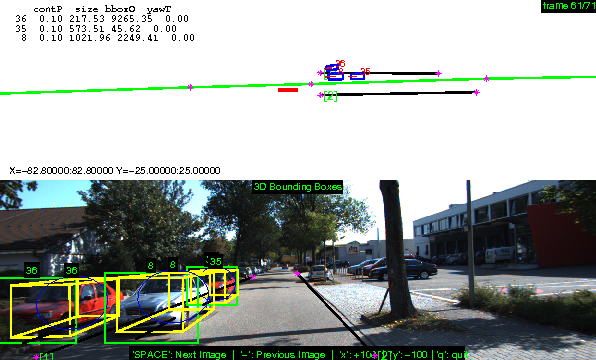
\includegraphics[width=\columnwidth]{results/0009_contPtTracks_size_bboxOcc_yawTstepWiseInference_0000000061.png}
  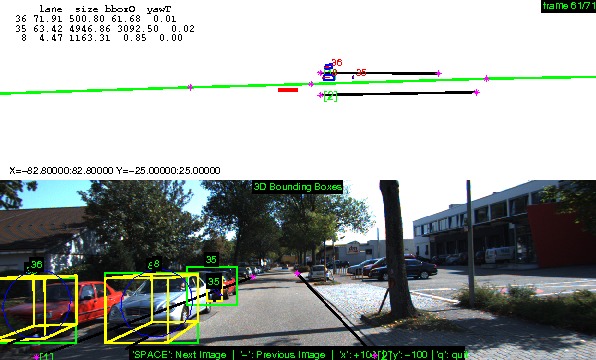
\includegraphics[width=\columnwidth]{results/0009_lane_size_bboxOcc_yawTstepWiseInference_0000000061.png}
  \caption{Qualitative localization results}
  \label{fig:qualLocalizationResults}
\end{figure}
\end{comment}


\end{document}
